% !TEX root = tutor-4-6-2.tex
% Edit tasks in task-4-6-2.tex.
\def\TutorEdition{1}
\expandafter\def\csname TutorSource507D42\endcsname{\href{https://ege.fipi.ru/bank/questions.php?search=1\&proj=BA1F39653304A5B041B656915DC36B38\&qid=507D42}{Источник: 507D42}}
\expandafter\def\csname TutorSource402B55\endcsname{\href{https://ege.fipi.ru/bank/questions.php?search=1\&proj=BA1F39653304A5B041B656915DC36B38\&qid=402B55}{Источник: 402B55}}
\expandafter\def\csname TutorSource2493F5\endcsname{\href{https://ege.fipi.ru/bank/questions.php?search=1\&proj=BA1F39653304A5B041B656915DC36B38\&qid=2493F5}{Источник: 2493F5}}
\expandafter\def\csname TutorSource7941\endcsname{\href{https://phys-ege.sdamgia.ru/problem?id=7941}{Источник: Решу ЕГЭ, №7941}}
\expandafter\def\csname TutorSource43830\endcsname{\href{https://phys-ege.sdamgia.ru/problem?id=43830}{Источник: Решу ЕГЭ, №43830}}
\expandafter\def\csname TutorSource50813\endcsname{\href{https://phys-ege.sdamgia.ru/problem?id=50813}{Источник: Решу ЕГЭ, №50813}}
\expandafter\def\csname TutorSource5177\endcsname{\href{https://phys-ege.sdamgia.ru/problem?id=5177}{Источник: Решу ЕГЭ, №5177}}
% !TEX root = task-4-6-2.tex
% Editable task bank. Append new BankTask blocks at the end of the document.
\documentclass[12pt,a4paper]{article}
\usepackage{physics-textbook}
\usepackage{graphicx,needspace}
\usetikzlibrary{decorations.pathmorphing}
\newif\ifShowSolutions
\ifdefined\TutorEdition
  \ShowSolutionstrue
\else
  \ShowSolutionsfalse % Change to \ShowSolutionstrue to display solutions.
\fi
\newcounter{banktask}
\newsavebox{\BankTaskBox}
\newcommand{\BankTaskContent}[3]{%
  \noindent\textbf{\thebanktask.}\quad #2\par
  \ifShowSolutions
    \Needspace{50mm}% Keep the solution heading with its opening text or diagram.
    #3\par
    \ifdefined\TutorEdition
      \ifcsname TutorSource#1\endcsname
        \nopagebreak\smallskip{\small\csname TutorSource#1\endcsname\par}%
      \fi
    \fi
  \fi
}
\newcommand{\BankTask}[3]{%
  \refstepcounter{banktask}\par\medskip
  \sbox{\BankTaskBox}{\begin{minipage}{\linewidth}%
    \BankTaskContent{#1}{#2}{#3}\end{minipage}}%
  \ifdim\dimexpr\ht\BankTaskBox+\dp\BankTaskBox\relax>\dimexpr\textheight-20mm\relax
    \Needspace{35mm}\BankTaskContent{#1}{#2}{#3}%
  \else
    \Needspace{\dimexpr\ht\BankTaskBox+\dp\BankTaskBox\relax}%
    \noindent\usebox{\BankTaskBox}\par
  \fi
  \medskip
}
\begin{document}
\BookSubsection{4.6.2}{Собирающая линза: действительное изображение предмета}


% Source 507D42: https://ege.fipi.ru/bank/questions.php?search=1&proj=BA1F39653304A5B041B656915DC36B38&qid=507D42
\BankTask{507D42}{
Предмет расположен на главной оптической оси тонкой собирающей линзы. Оптическая сила линзы \(D=5\,\text{дптр}\). Изображение предмета действительное, увеличение (отношение высоты изображения предмета к высоте самого предмета) \(k=2\). Найдите расстояние между предметом и его изображением. Ответ выразите в сантиметрах. (в $\text{см}$).
}{
\smallskip\noindent\textbf{Решение от GPT}\par
Фокусное расстояние \(F=1/D=0{,}2\,\text{м}=20\,\text{см}\). Обозначим расстояния от линзы до предмета и изображения через \(a\) и \(b\). Тогда \(b/a=k=2\), а по формуле тонкой линзы
\[\frac1F=\frac1a+\frac1b=\frac{3}{2a}.\]
Отсюда \(a=30\,\text{см}\), \(b=60\,\text{см}\). Предмет и действительное изображение находятся по разные стороны линзы, поэтому \(l=a+b=90\,\text{см}\). Ответ: \(90\,\text{см}\).
}

% Source 402B55: https://ege.fipi.ru/bank/questions.php?search=1&proj=BA1F39653304A5B041B656915DC36B38&qid=402B55
\BankTask{402B55}{
Предмет высотой \(6\,\text{см}\) расположен на горизонтальной главной оптической оси тонкой собирающей линзы. Оптическая сила линзы \(5\,\text{дптр}\). Действительное изображение предмета находится на расстоянии \(30\,\text{см}\) от оптического центра линзы. Найдите высоту изображения предмета. (в $\text{см}$).
}{
\smallskip\noindent\textbf{Решение от GPT}\par
Фокусное расстояние линзы \(F=1/D=0{,}2\,\text{м}=20\,\text{см}\). По формуле тонкой линзы расстояние до предмета
\[
a=\frac{Fb}{b-F}=\frac{20\cdot30}{30-20}=60\text{ см}.
\]
Высота изображения \(H=h\,b/a=6\cdot30/60=3\,\text{см}\). Изображение перевёрнутое.
\(\boxed{3\text{ см}}\).
}

% Source 2493F5: https://ege.fipi.ru/bank/questions.php?search=1&proj=BA1F39653304A5B041B656915DC36B38&qid=2493F5
\BankTask{2493F5}{
Необходимо собрать экспериментальную установку, с помощью которой можно определить оптическую силу собирающей линзы. В качестве источника света школьник взял горящую свечу. Какие два предмета из приведённого ниже перечня оборудования необходимо дополнительно использовать для проведения этого эксперимента?
\begin{enumerate}
\item гальванометр
\item линейка
\item экран
\item зеркало
\item динамометр
\end{enumerate}
}{
\smallskip\noindent\textbf{Решение от GPT}\par
На экране (3) получают резкое изображение свечи, а линейкой (2) измеряют расстояния от свечи до линзы \(a\) и от линзы до экрана \(b\). Оптическая сила линзы \(D=1/F=1/a+1/b\); при расстояниях в метрах она выражается в диоптриях. Гальванометр (1) измеряет силу тока, зеркало (4) для этого опыта не требуется, динамометр (5) измеряет силу. Ответ: 2, 3.
}

% Source 7941: https://phys-ege.sdamgia.ru/problem?id=7941
\BankTask{7941}{
\begin{center}\begin{tikzpicture}[>=stealth,line width=.55pt]\draw(-3.9,0)--(3.48,0);\draw[<->,thick](0,-1.65)--(0,1.65)node[above left]{Л};\draw[->](-3.08,0)--(-3.08,.91)node[above]{$B$};\node[below]at(-3.08,0){$A$};\end{tikzpicture}\end{center}С помощью тонкой линзы на экране получают изображение объекта AB, расположенного параллельно ей. После чего линзу закрывают ободком из черного картона. Нарисуйте ход лучей и объясните, что произойдет с изображением на экране.
}{
\smallskip\noindent\textbf{Решение}\par
\begin{center}\begin{tikzpicture}[>=stealth,line width=.55pt]\draw(-3.9,0)--(3.48,0);\draw[<->,thick](0,-1.65)--(0,1.65)node[above left]{Л};\draw[->](-3.08,0)--(-3.08,.91)node[above]{$B$};\node[below]at(-3.08,0){$A$};\draw[->](2.42,0)--(2.42,-.71)node[below]{$B\prime$};\node[above]at(2.42,0){$A\prime$};\foreach \y in {-1.2,-.88,-.56,-.27,0,.28,.58,.91,1.2}{\draw[orange!85!black,line width=.35pt](-3.08,.91)--(0,\y)--(2.42,-.71);}\node[above]at(1.35,0){$F$};\node[left]at(-3.12,.46){$a$};\node[below]at(-1.48,0){$x$};\node[below]at(1.92,0){$y$};\node[right]at(2.49,-.38){$b$};\end{tikzpicture}\end{center}Изображение было получено на экране, значит, оно действительное, а объект AB расположен от линзы на расстоянии больше фокусного. Построим изображение A'B'. Луч, идущий параллельно главной оптической оси, после преломления в линзе проходит через фокус, а луч, прошедший через пересечение главной оптической оси и линзы, не преломляется. Пересечение лучей дает точку B'. Все прочие лучи, идущие от B и преломляющиеся в линзе, также проходят через точку B'. 
Запишем уравнение тонкой линзы:

\[\frac{1}{F} = \frac{1}{x} + \frac{1}{y} \Longleftrightarrow y= \frac{xF}{x - F} ,\]

где x  — расстояние от объекта до линзы, y  — расстояние от линзы до изображения, F  — фокусное расстояние линзы. Расстояние y не зависит от высоты объекта, значит, изображение A'B' перпендикулярно главной оптической оси. Из построения получаем, что изображение перевернутое.
\begin{center}\begin{tikzpicture}[>=stealth,line width=.55pt]\draw(-3.9,0)--(3.48,0);\draw[<->,thick](0,-1.65)--(0,1.65)node[above left]{Л};\draw[->](-3.08,0)--(-3.08,.91)node[above]{$B$};\node[below]at(-3.08,0){$A$};\draw[->](2.42,0)--(2.42,-.71)node[below]{$B\prime$};\node[above]at(2.42,0){$A\prime$};\foreach \y in {-.86,-.58,-.29,0,.29,.58,.86}{\draw[orange!85!black,line width=.35pt](-3.08,.91)--(0,\y)--(2.42,-.71);}\foreach \y in {-1.22,-1.04,1.04,1.22}{\draw[orange!85!black,line width=.35pt](-3.08,.91)--(0,\y);}\draw[orange!80!black,line width=3pt](-.04,.93)--(-.04,1.39) (-.04,-.93)--(-.04,-1.39);\end{tikzpicture}\end{center}Размер изображения можно найти из подобия треугольников:

\[\frac{a}{b} = \frac{x}{y} \Longleftrightarrow b= \frac{ay}{x} .\]

После того как линзу закрыли ободком, часть лучей стала поглощаться картоном. Ход непоглощенных лучей остался без изменения. Следовательно, изображение на экране останется на месте, только будет тусклее.
}

% Source 43830: https://phys-ege.sdamgia.ru/problem?id=43830
\BankTask{43830}{
\begin{center}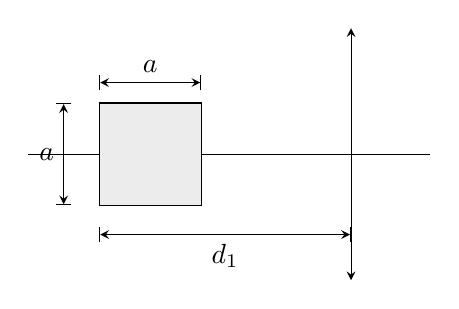
\begin{tikzpicture}[>=stealth]

\draw (-4.1,0)--(1,0);\draw[<->](0,-1.6)--(0,1.6);
\draw[fill=gray!15](-3.2,-.65)rectangle(-1.9,.65);
\draw[|<->|](-3.2,.91)--(-1.9,.91)node[midway,above]{$a$};
\draw[|<->|](-3.65,-.65)--(-3.65,.65)node[midway,left]{$a$};
\draw[|<->|](-3.2,-1.02)--(0,-1.02)node[midway,below]{$d_1$};
\end{tikzpicture}\end{center}
Квадрат со стороной a  =  $20\,\text{см}$ расположен в плоскости главной оптической оси тонкой собирающей линзы с оптической силой D  =  $2\,\text{дптр}$ так, что две его стороны параллельны плоскости линзы (см. рис.). Расстояние от дальней стороны квадрата до плоскости линзы $d_{1}$  =  $90\,\text{см}$. Определите площадь изображения квадрата в линзе. Сделайте рисунок, на котором постройте изображение квадрата в линзе, указав ход всех необходимых для построения лучей.
}{
\smallskip\noindent\textbf{Решение}\par
Обозначим вершины квадрата ABCD, тогда AB  =  AD  =  a.  
Для построения изображения квадрата проведём побочные оптические оси AO и BO, а также луч AB, параллельный главной оптической оси, который, преломившись, пройдёт через фокус линзы. В силу симметрии предмета относительно главной оптической оси его изображение также будет симметричным. В результате построений получим изображение квадрата ABCD в виде равнобедренной трапеции $A_{1}$$B_{1}$$C_{1}$$D_{1}$ (см. рис.).
\begin{center}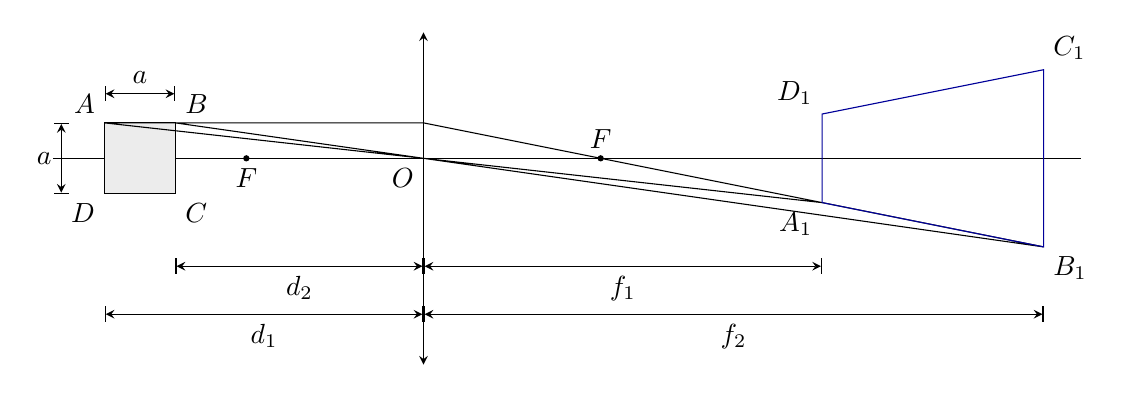
\begin{tikzpicture}[>=stealth]

\draw (-4.7,0)--(8.35,0);\draw[<->](0,-2.62)--(0,1.6);\node[below left] at(0,0){$O$};
\draw[fill=gray!15](-4.05,-.45)rectangle(-3.15,.45);
\node[above left]at(-4.05,.45){$A$};\node[above right]at(-3.15,.45){$B$};
\node[below right]at(-3.15,-.45){$C$};\node[below left]at(-4.05,-.45){$D$};
\fill (-2.25,0)circle(.04) node[below]{$F$} (2.25,0)circle(.04)node[above]{$F$};
\draw (-4.05,.45)--(0,.45)--(7.875,-1.125) (-4.05,.45)--(5.0625,-.5625) (-3.15,.45)--(7.875,-1.125);
\draw[blue!60!black] (5.0625,-.5625)--(7.875,-1.125)--(7.875,1.125)--(5.0625,.5625)--cycle;
\node[below left]at(5.0625,-.5625){$A_1$};\node[below right]at(7.875,-1.125){$B_1$};
\node[above right]at(7.875,1.125){$C_1$};\node[above left]at(5.0625,.5625){$D_1$};
\draw[|<->|](-4.05,.82)--(-3.15,.82)node[midway,above]{$a$};
\draw[|<->|](-4.6,-.45)--(-4.6,.45)node[midway,left]{$a$};
\draw[|<->|](-3.15,-1.37)--(0,-1.37)node[midway,below]{$d_2$};
\draw[|<->|](0,-1.37)--(5.0625,-1.37)node[midway,below]{$f_1$};
\draw[|<->|](-4.05,-1.98)--(0,-1.98)node[midway,below]{$d_1$};
\draw[|<->|](0,-1.98)--(7.875,-1.98)node[midway,below]{$f_2$};
\end{tikzpicture}\end{center}

Согласно формуле оптической силы линзы $F = \frac{1}{D} = \frac{1}{2} = 0{,}5 \,\text{м} = 50 \,\text{см}.$ Расстояние от линзы до квадрата равно $d_2 = d_1 - a = 90 - 20 = 70 \,\text{см}.$ По формуле тонкой линзы определим расстояния от линзы до оснований трапеции:

$\frac{1}{F} = \frac{1}{d_1} + \frac{1}{f_1} ,$
$\frac{1}{F} = \frac{1}{d_2} + \frac{1}{f_2} .$

 В итоге

$f_1 = \frac{Fd_1}{d_1 - F} = \frac{50 \cdot 90}{90 - 50} = 112{,}5 \,\text{см},$
$f_2 = \frac{Fd_2}{d_2 - F} = \frac{50 \cdot 70}{70 - 50} = 175 \,\text{см}.$

 Высота трапеции $h = f_2 - f_1 = 62{,}5 \,\text{см}.$
Используя формулу увеличения линзы для двух сторон квадрата, получим

$\frac{AD}{d_1} = \frac{A_1D_1}{f_1} ,$
$\frac{BC}{d_2} = \frac{B_1C_1}{f_2} .$

 Следовательно,

$A_1D_1 = \frac{f_1 \cdot AD}{d_1} = \frac{112{,}5 \cdot 20}{90} = 25 \,\text{см},$
$B_1C_1 = \frac{f_2 \cdot BC}{d_2} = \frac{175 \cdot 20}{70} = 50 \,\text{см}.$

Площадь изображения (трапеции) определяется формулой

\[S = \frac{A_1D_1 + B_1C_1}{2} \cdot h = \frac{25 + 50}{2} \cdot 62{,}5 \approx 2344 \,\text{см} ^2 .\]

Ответ: $S \approx 2344 \,\text{см} ^2 .$
}

% Source 50813: https://phys-ege.sdamgia.ru/problem?id=50813
\BankTask{50813}{
Линза, фокусное расстояние которой $30\,\text{см}$, даёт на экране резкое изображение предмета c пятикратным увеличением. Экран пододвинули к линзе вдоль её главной оптической оси. Затем при неизменном положении линзы передвинули предмет на $3\,\text{см}$ так, чтобы изображение снова стало резким. На какое расстояние сдвинули экран относительно его первоначального положения? Сделайте рисунок построения изображений в линзе с указанием хода лучей.
}{
\smallskip\noindent\textbf{Решение}\par
Построим изображение предмета в собирающей линзе в первом случае:


\begin{center}\begin{tikzpicture}[>=stealth,line width=.65pt]\draw (-2.1,0)--(7.95,0);\draw[<->](0,-2.55)--(0,2.55);\draw[cyan!50,line width=2.5pt](7.5,-2.48)--(7.5,2.46);\node[below]at(7.5,-2.5){Экран};\draw[->,orange!80!black](-1.5,0)node[below left]{$B$}--(-1.5,.35)node[above left]{$A$};\draw[->,red!70!black](7.5,0)node[below left]{$C$}--(7.5,-1.75)node[below left]{$D$};\draw[green!55!black](-1.5,.35)--(0,.35)--(7.5,-1.75) (-1.5,.35)--(7.5,-1.75);\draw[->,green!55!black](-1,.35)--(-.64,.35);\draw[->,green!55!black](1.8,{-.35*1.8/1.5})--(2.14,{-.35*2.14/1.5});\draw[->,green!55!black](2.65,{.35-.28*2.65})--(3,{.35-.28*3});\fill(-1.25,0)circle(.026)node[below right]{$F$};\fill(1.25,0)circle(.026)node[above]{$F$};\node[below left]at(0,0){$O$};\draw[thin](-1.5,.38)--(-1.5,2.15);\draw[<->](-1.5,2.1)--(0,2.1)node[midway,above]{$d_1$};\draw[<->](0,2.1)--(7.5,2.1)node[midway,above]{$f_1$};\end{tikzpicture}\end{center}


Используем формулы тонкой линзы $\frac{1}{d_1} + \frac{1}{f_1} = \frac{1}{F}$ и увеличения, даваемого собирающей линзой, $\Gamma = \frac{f_1}{d_1} .$ Из них находим расстояние от предмета до линзы и от изображения до линзы: $d_1 = 1{,}2F,$ $f_1 = 6F.$
Построим изображение предмета в собирающей линзе во втором случае:


\begin{center}\begin{tikzpicture}[>=stealth,line width=.65pt]\draw (-2.1,0)--(7.95,0);\draw[<->](0,-2.55)--(0,2.55);\draw[cyan!50,line width=2.5pt](5.4167,-2.48)--(5.4167,2.46);\node[below]at(5.4167,-2.5){Экран};\draw[->,orange!80!black](-1.625,0)node[below left]{$B$}--(-1.625,.35)node[above left]{$A$};\draw[->,red!70!black](5.4167,0)node[below left]{$C_1$}--(5.4167,-1.166673846153846)node[below left]{$D_1$};\draw[green!55!black](-1.625,.35)--(0,.35)--(5.4167,-1.166673846153846) (-1.625,.35)--(5.4167,-1.166673846153846);\draw[->,green!55!black](-1,.35)--(-.64,.35);\draw[->,green!55!black](1.8,{-.35*1.8/1.625})--(2.14,{-.35*2.14/1.625});\draw[->,green!55!black](2.65,{.35-.28*2.65})--(3,{.35-.28*3});\fill(-1.25,0)circle(.026)node[below right]{$F$};\fill(1.25,0)circle(.026)node[above]{$F$};\node[below left]at(0,0){$O$};\draw[thin](-1.625,.38)--(-1.625,2.15);\draw[<->](-1.625,2.1)--(0,2.1)node[midway,above]{$d_2$};\draw[<->](0,2.1)--(5.4167,2.1)node[midway,above]{$f_2$};\draw[dashed](-1.5,0)--(-1.5,2.15) (7.5,-2.3)--(7.5,2.22);\draw[<->](-1.5,1.68)--(-1.625,1.68)node[midway,left=.24cm]{$\Delta d$};\draw[<->](5.4167,2.1)--(7.5,2.1)node[midway,above]{$x$};\end{tikzpicture}\end{center}


При этом видно, что если по условию расстояние от линзы до экрана уменьшили на величину x, то расстояние от предмета до линзы увеличилось на величину $\Delta d.$ Запишем формулу собирающей линзы для этого случая:

$\frac{1}{d_2} + \frac{1}{f_2} = \frac{1}{F} ,$
$\frac{1}{d_1 + \Delta d} + \frac{1}{f_1 - x} = \frac{1}{F} ,$
$\frac{1}{1{,}2F + \Delta d} + \frac{1}{6F - x} = \frac{1}{F} ,$

откуда находим искомое расстояние:

\[x = \frac{5F \Delta d}{0{,}2F + \Delta d} = \frac{5 \cdot 30 \cdot 3}{0{,}2 \cdot 30 + 3} = 50 \,\text{см}.\]

Ответ: $50\,\text{см}$.
}

% Source 5177: https://phys-ege.sdamgia.ru/problem?id=5177
\BankTask{5177}{
\begin{center}\begin{tikzpicture}[>=stealth,line width=.65pt]\draw(-3.75,0)--(2.95,0);\draw[<->](0,-1.95)--(0,1.95);\draw[orange!80!black](-3.4,0)--(-2.3,1.1)--(-2.3,0)--cycle;\foreach \x/\l in {-3.4/2F,-1.7/F,1.7/F}{\fill (\x,0)circle(.035)node[below]{$\l$};}\node[above left]at(-3.4,0){$A$};\node[above left]at(-2.3,1.1){$B$};\node[above right]at(-2.3,0){$C$};\end{tikzpicture}\end{center}

 Равнобедренный	прямоугольный треугольник ABC расположен перед тонкой собирающей линзой оптической силой $2{,}5\,\text{дптр}$ так, что его катет АС лежит на главной оптической оси линзы (см. рисунок). Вершина прямого угла С лежит ближе к центру линзы, чем вершина острого угла А. Расстояние от центра линзы до точки А равно удвоенному фокусному расстоянию линзы, АС = $4\,\text{см}$. Постройте изображение треугольника и найдите площадь получившейся фигуры.
}{
\smallskip\noindent\textbf{Решение}\par
Изображение треугольника построено на рисунке. 


\begin{center}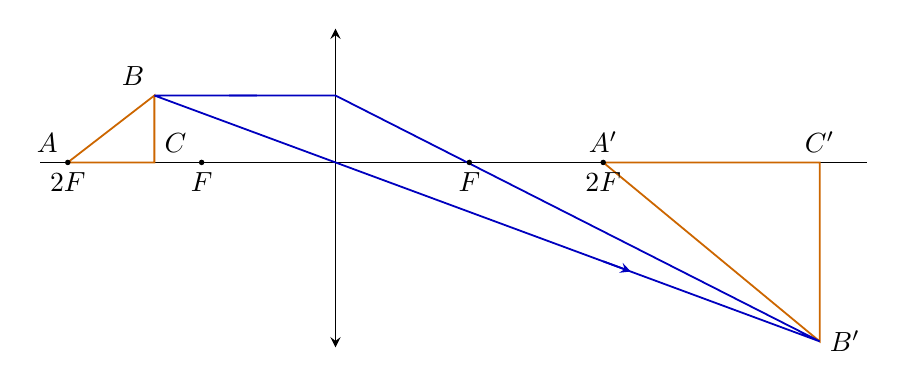
\begin{tikzpicture}[>=stealth,line width=.65pt]\draw(-3.75,0)--(6.75,0);\draw[<->](0,-2.35)--(0,1.7);\draw[orange!80!black](-3.4,0)--(-2.3,.85)--(-2.3,0)--cycle (3.4,0)--(6.15,-2.273)--(6.15,0)--cycle;\draw[blue!75!black](-2.3,.85)--(0,.85)--(6.15,-2.273) (-2.3,.85)--(6.15,-2.273);\draw[->,blue!75!black](-1.35,.85)--(-1,.85) (3.4,-1.256)--(3.75,-1.385);\foreach \x/\l in {-3.4/2F,-1.7/F,1.7/F,3.4/2F}{\fill (\x,0)circle(.035)node[below]{$\l$};}\node[above left]at(-3.4,0){$A$};\node[above left]at(-2.3,.85){$B$};\node[above right]at(-2.3,0){$C$};\node[above]at(3.4,0){$A^{\prime}$};\node[above]at(6.15,0){$C^{\prime}$};\node[right]at(6.15,-2.273){$B^{\prime}$};\end{tikzpicture}\end{center}


Изображение точки B удобно найти как пересечение луча, проходящего через центр линзы и луча, падающего на линзу параллельно главной оптической оси.
Изображение точки С находится в точности под изображением точки В. Положение изображения точки А легко определить из формулы тонкой линзы: 

\[\frac{1}{d} + \frac{1}{f} = \frac{1}{F}\]

Поскольку точка А находится в двойном фокусе, то $d=2F,$ а значит, и $f=2F,$ то есть изображение точки А также находится в двойном фокусе.
Наконец, легко понять, что изображение треугольника вновь будет треугольником. Действительно, если пропустить луч через сторону ВА, то после преломления на этом луче будут находиться изображения всех точек со стороны ВА, то есть гипотенуза прямоугольного треугольника перейдет в гипотенузу треугольника-изображения.

Определим фокусное расстояние

\[F= \frac{1}{D} = \frac{1}{2{,}5\,\text{дптр}} =0{,}4\,\text{м}.\]

Обозначим катет треугольника ABC через $h.$
Найдем расстояние от линзы до изображения точки С ($d=2F - h$):

\[f= \frac{dF}{d - F} = \frac{( 2 \cdot 40 \,\text{см} - 4\,\text{см} ) \cdot 40\,\text{см}}{2 \cdot 40 \,\text{см} - 4\,\text{см} - 40\,\text{см}} \approx 84{,}4\,\text{см}.\]

Горизонтальный катет равен 

\[a=f - 2F\approx 4{,}4\,\text{см}.\]

Из подобия треугольников для вертикального катета треугольника-изображения имеем

\[\frac{h}{b} = \frac{d}{f} \Longleftrightarrow b= \frac{hf}{2F - h} \approx 4{,}4 \,\text{см}.\]

Таким образом, площадь треугольника изображения равна: 

\[S' = \frac{1}{2} ab = \frac{1}{2} ( 4{,}4\,\text{см} ) ^2 \approx 10\,\text{см} ^2 .\]

Ответ: $10\,\text{см} ^2$

Примечание:
В решение можно было использовать тот факт, что треугольник-изображение также является равнобедренным. Это следует из того факта, что луч, проходящий через двойной фокус после преломления в линзе снова попадет в двойной фокус. Тем самым после преломления в линзе луч идет по тем же самым углом к главной оптической оси, что и до преломления в линзе. Поскольку в нашем случае этот угол равен $45 ^\circ,$ то равнобедренный треугольник снова получится равнобедренным.
}

\end{document}

